\documentclass[11pt]{beamer}
\usetheme{Boadilla}
\usepackage[utf8]{inputenc}
\usepackage{amsmath}
\usepackage{amsfonts}
\usepackage{amssymb}
\usepackage{graphicx}
\usepackage{listings}
\usepackage{verbatim}
\usepackage[spanish]{babel}
%\author{}
%\title{}
%\setbeamercovered{transparent}
%\setbeamertemplate{navigation symbols}{}
%\logo{}
%\institute{}
%\date{}
%\subject{}
\begin{document}

\begin{frame}
\titlepage
\end{frame}

\begin{frame}
\tableofcontents
\end{frame}

\begin{frame}{Acerca de MarkDown}

Es un lenguaje de marcado creado para escribir en la web de tal manera que es fácil de editar y de leer a la vez.

Usualmente todo texto escito en Markdown se suele compilar en HTML, un compilador de Markdown a Latex nos serviría de utilidad para publicar un informe en la web como para presentarlo formalmente en un informe.
\begin{center}

\includegraphics[scale=0.2]{imagenes/markdown-512.png} 
\end{center}
\end{frame}

\begin{frame}{Comparación entre Latex y Markdown}
\begin{center}
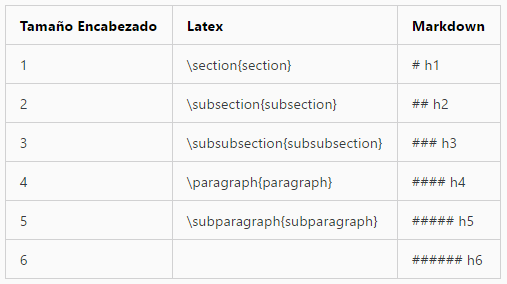
\includegraphics[scale=0.8]{imagenes/com.png} 
\end{center}
\end{frame}


\end{document}
